\section{Extracción de características}\label{sec:features}

\begin{frame}
    \frametitle{Extracción de características}

    \begin{columns}
        \column{0.5\textwidth}

        \begin{figure}[!h]
            \centering
            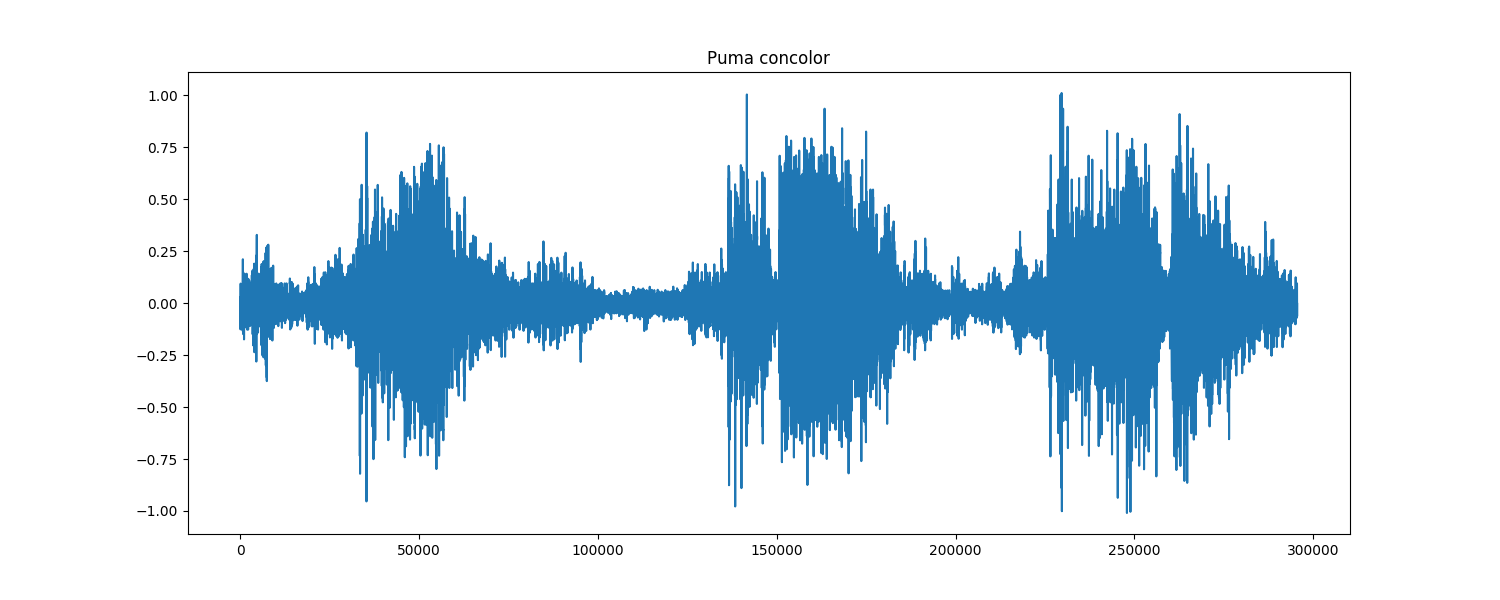
\includegraphics[width=\textwidth]{oscillogram.png}
        \end{figure}
        \begin{figure}[!h]
            \centering
            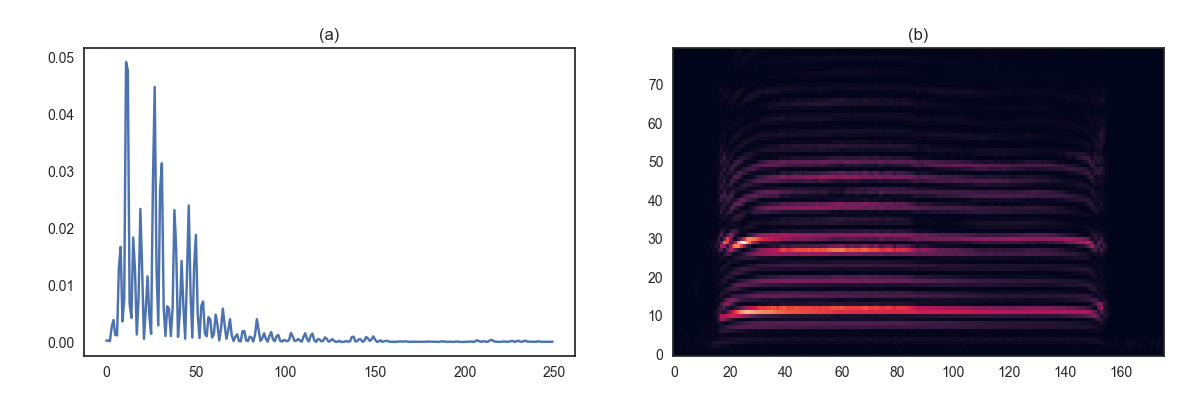
\includegraphics[width=\textwidth]{spectrum+spectrogram.png}
        \end{figure}

        \column{0.5\textwidth}

        Hello, World!

    \end{columns}
\end{frame}

\begin{frame}
    \frametitle{Características temporales}

    \begin{columns}
        \column{0.5\textwidth}

        \begin{figure}[!h]
            \centering
            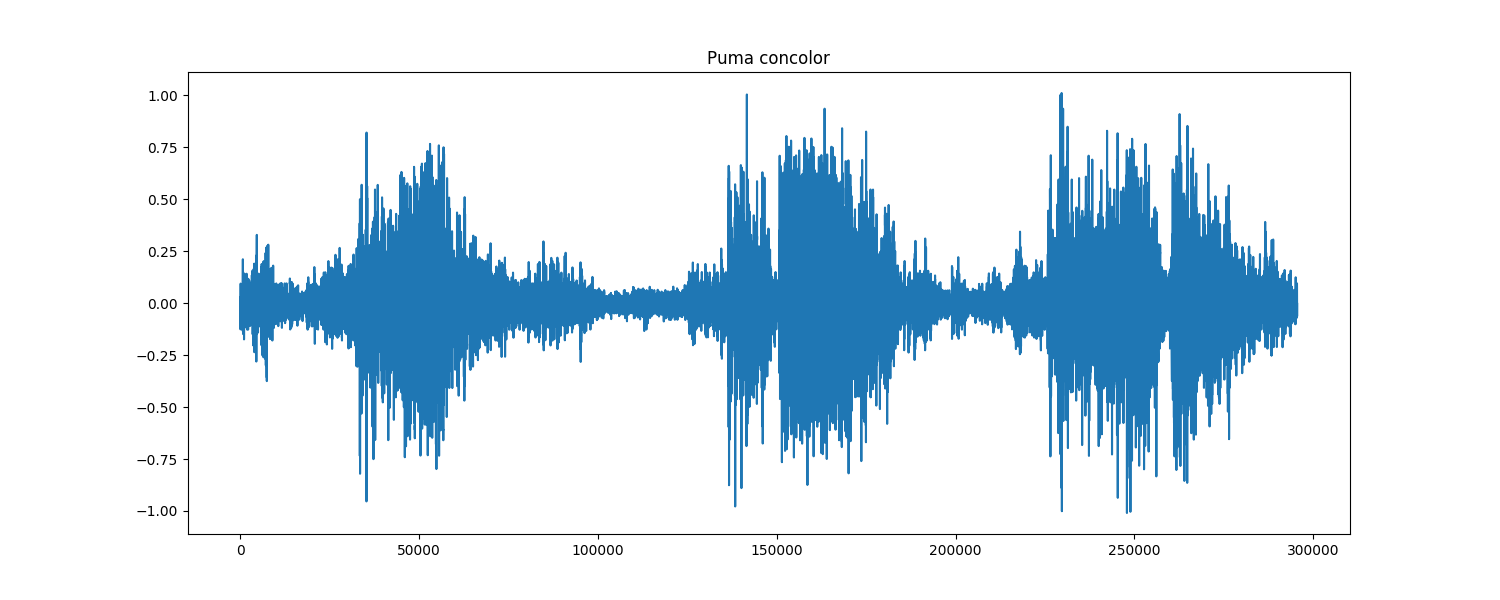
\includegraphics[width=\textwidth]{oscillogram.png}
        \end{figure}
        \begin{figure}[!h]
            \centering
            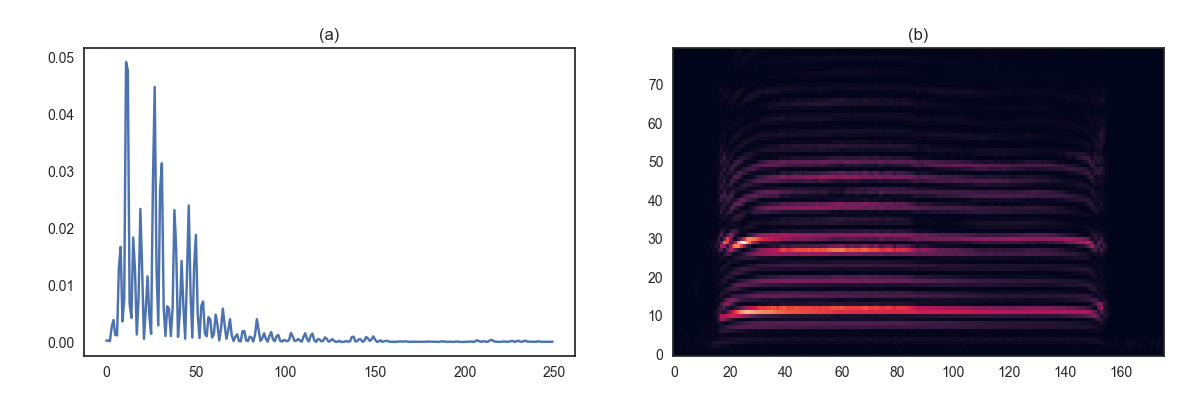
\includegraphics[width=\textwidth]{spectrum+spectrogram.png}
        \end{figure}

        \column{0.5\textwidth}

        Hello, World!

    \end{columns}
\end{frame}

\begin{frame}
    \frametitle{Características espectrales}

\end{frame}

\begin{frame}
    \frametitle{Características armónicas}

\end{frame}

\begin{frame}
    \frametitle{Mel Frequency Cepstral Coefficients}

\end{frame}